\documentclass{report}
\usepackage[T1]{fontenc}
\usepackage[utf8]{inputenc}
\usepackage[backend=biber, style=ieee]{biblatex}
\usepackage{csquotes}
\usepackage[portuguese]{babel}
\usepackage{blindtext}
\usepackage[printonlyused]{acronym}
\usepackage{hyperref}
\usepackage{graphicx}
\usepackage{indentfirst}
\usepackage{tabularx}
\usepackage{float}
\usepackage{subcaption}

%%\bibliography{bibliografia}
%%\setlength{\parskip}{0.39em}
%%\newcommand{\centered}[1]{\begin{tabular}{l} #1 \end{tabular}}


%For the header and footer
\usepackage{fancyhdr}
\fancypagestyle{plain}{%
\fancyfoot[L]{\emph{Departamento de Eletrónica, Telecomunicações e Informática }} % except the center
\fancyfoot[R]{\thepage{}}
\renewcommand{\headrulewidth}{0.4pt}
\renewcommand{\footrulewidth}{0.4pt}
}
\pagestyle{fancy}
\rhead{\emph{Projeto Final LABI2022G5}}
\fancyfoot[LO,L]{\emph{Departamento de Eletrónica, Telecomunicações e Informática }}
\cfoot{}
\fancyfoot[RO, RE]{\thepage}
\renewcommand{\headrulewidth}{0.1pt}
\renewcommand{\footrulewidth}{0.1pt}
%For the header and footer Over

%Page Border
\usepackage{pgf}
\usepackage{pgfpages}

\pgfpagesdeclarelayout{boxed}
{
  \edef\pgfpageoptionborder{0pt}
}
{
  \pgfpagesphysicalpageoptions
  {%
    logical pages=1,%
  }
  \pgfpageslogicalpageoptions{1}
  {
    border code=\pgfsetlinewidth{2pt}\pgfstroke,%
    border shrink=\pgfpageoptionborder,%
    resized width=.95\pgfphysicalwidth,%
    resized height=.95\pgfphysicalheight,%
    center=\pgfpoint{.5\pgfphysicalwidth}{.5\pgfphysicalheight}%
  }%
}
\pgfpagesuselayout{boxed}
\setlength{\parindent}{1cm}




\begin{document}
%%% DEFINIÇÕES GLOBAIS %%%
\def\titulo{Projeto Final LABI2022}
\def\data{Aveiro, julho 2021}
\def\autoresa{Miguel Vila, Diogo Silva}
\def\autoresb{Miguel Reis, Martim Carvalho}
\def\autoresacontactos{(107276) \href{mailto:miguelovila@ua.pt}{miguelovila@ua.pt}, (108212) \href{mailto:dsgps@ua.pt}{dsgps@ua.pt}}
\def\autoresbcontactos{(108545) \href{mailto:mreis@ua.pt}{mreis@ua.pt}, (108749) \href{mailto:martimhcarvalho@ua.pt}{martimhcarvalho@ua.pt}}
\def\projetocodeua{\url{http://code.ua.pt/projects/labi2022g5}}
\def\departamento{DETI}
\def\empresa{UNIVERSIDADE DE AVEIRO}
\def\logotipo{ua.pdf}

%%% ESTRUTURA CAPA %%%
\begin{titlepage}
\begin{center}
\vspace*{20mm}
{\Huge \titulo}\\ 
\vspace{10mm}
{\Large \empresa}\\
\vspace{10mm}
{\LARGE \autores}\\ 
\vspace{30mm}
\begin{figure}[h]
\center
\includegraphics{\logotipo}
\end{figure}
\vspace{20mm}
\end{center}
\begin{flushright}
\end{flushright}
\end{titlepage}

%%%  PÁGINA DE TÍTULO %%%
\begin{titlepage}
\title{%
{\Huge\textbf{\titulo}}\\
{\Large \departamento\\ \empresa}
}
\author{
  \autoresa\\\
  \autoresacontactos\\\\
  \autoresb\\\
  \autoresbcontactos\\\\
  \projetocodeua
}
\date{\data}
\maketitle
\pagenumbering{arabic}
\end{titlepage}


\tableofcontents

%%% OBJETIVOS %%%
\renewcommand{\abstractname}{OBJETIVOS DO PROJETO}
\begin{abstract}

Neste trabalho foi-nos solicitado a realização de um site online com a finalidade de os seus utilizadores poderem armazenar e trocar as suas imagens de forma rápida e intuitiva. 

Além de poderem ser armazenadas imagens pré-existentes, os utilizadores poderão tambem publicar no site as suas próprias criacões, formando uma coleção visivel a qualquer utilizador, e disponivel para ser requisitada por qualquer um que esteja registado no site.
Todas as imagens colocadas no site serão sujeitas a uma marca de agua gerada automaticamente, como tambem o logo do mesmo com o objetivo de garantir a autenticidade das mesmas.

Comforme o anteriormente exposto, ao ser adicionada uma imagem pelo utilizador o seu nome estará associado há imagem e visível no site, impossibilitando assim o plágio de imagens.

Em relação às trocas entre diversos utilizadores, foi desenvolvido um sistema de encriptação de forma a garantir a segurança das imagens, para que as imagens possam ser trocadas e não roubas. Assim estas trocas, para além de seguras, são tambem instântanias e simples, tendo apenas o utilizador que aceder à sua coleção, escolher a imagem e por fim digitar o seu destinatário.

\end{abstract}


\chapter{Interface Web}
Esta componente é a responsável pelo registo de novos utilizadores e pelo login dos mesmos. Após o registo no nosso site com um nome de utilizador, será gerada automaticamente uma palavra-passe para cada utilizador usar no seu login e ter acesso ao site pela sua conta.

Ao logar-se com a sua conta, o utilizador terá acesso a uma lista de coleções de imagens, colocadas no site por outros usuários, e disponiveis para serem requisitadas por qualquer utilizador que as queira adicionar a sua coleção. 

O utilizador terá também acesso à pagina do seu perfil pessoal, onde estarão lá colocadas todas as imagens que pertencem à sua coleção pessoal. Nesta mesma pagina será possivel enviar as suas imagens a outros usuários do site, apenas digitando o seu nome de utilizador na imagem que quer enviar. 

Além de armazenar as suas coleções requisitadas, o utilizador também poderá ter acesso a página "Carregar" onde poderá, de maneira intuitiva, colocar as suas proprias criações no site, de modo a serem partilhadas com todos os outros usuários do mesmo. Estas imagens adicionadas poderão ser requisitadas pelos outros utilizadores como qualquer outra imagem que pertença ao site.

Por fim podem observar na nossa Navbar, na pagina inicial possui uma aba "Sobre", onde pode encontrar um resumo do objetivo do site e também os participantes com os seus respetivos contactos. 
\begin{figure}[H]
    \centering
    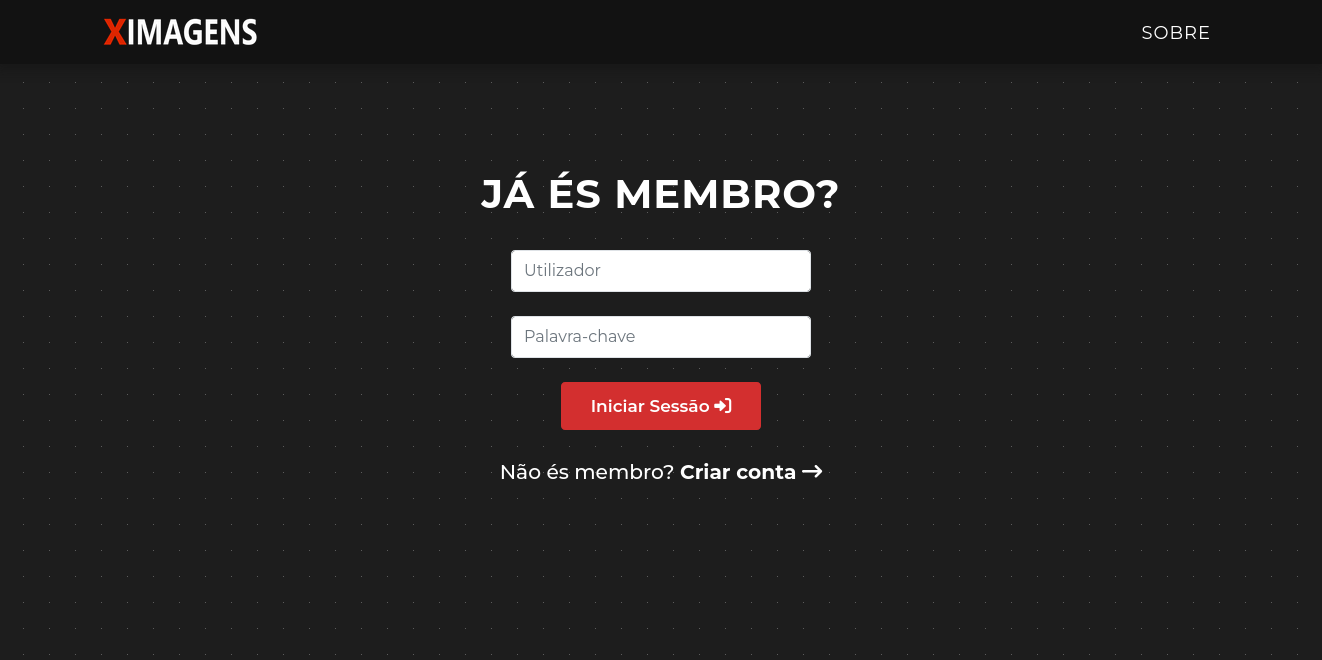
\includegraphics[width=\textwidth]{unknoawn.png}
    \caption{Página de início de sessão}
\end{figure}
\begin{figure}[H]
    \centering
    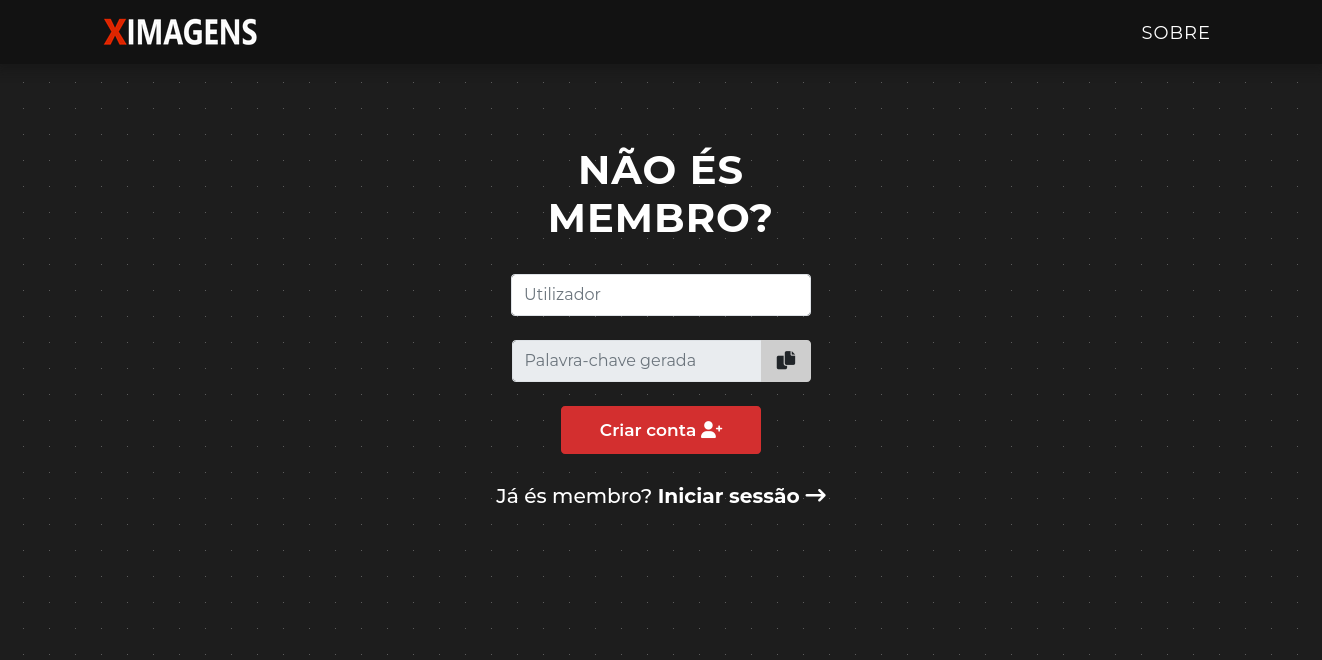
\includegraphics[width=\textwidth]{newuser.png}
    \caption{Página de criar Utilizador}
\end{figure}

\begin{figure}[H]
    \centering
    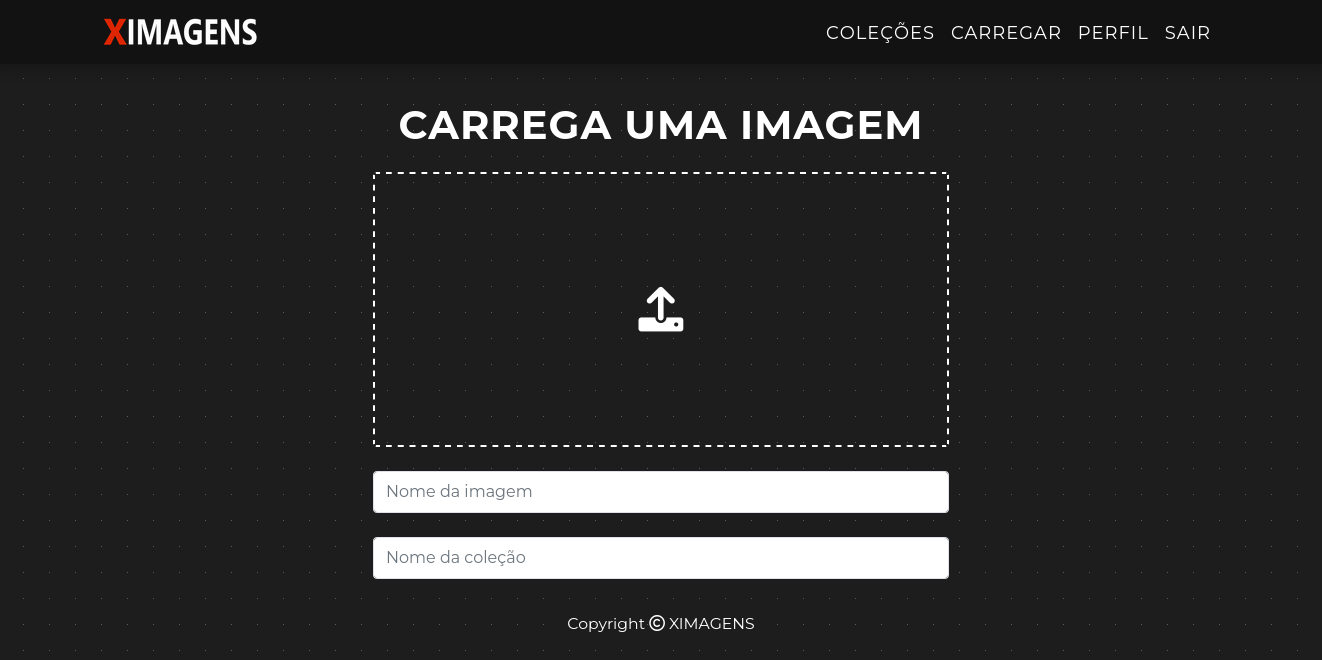
\includegraphics[width=\textwidth]{upload.png}
    \caption{Página para o utilizador dar upload das suas imagens}
\end{figure}


\chapter{Aplicação Web}
No nosso site a aplicação web foi desenvolvida com o intuito de tornar o site o mais apelativo, minimalista e intuitivo ao utilizador de modo a não surgirem muitas duvidas na sua utilização, o que poderia levar ao desuso do mesmo. 

Assim, a base deste site e que o sustenta, consiste em python, uma linguagem nos irá servir conteúdos estáticos, nomeadamente HTML, CSS e JS, que permitem a navegação entre os diversos componentes da interface do site.

Ainda foi desenvolvida uma intface programática, responsiva com objetos JSON e que além disso permite obter e inserir informação sobre as imagens, autores e comentários realizados prlos utilizadores do site.

\begin{figure}[H]
    \centering
    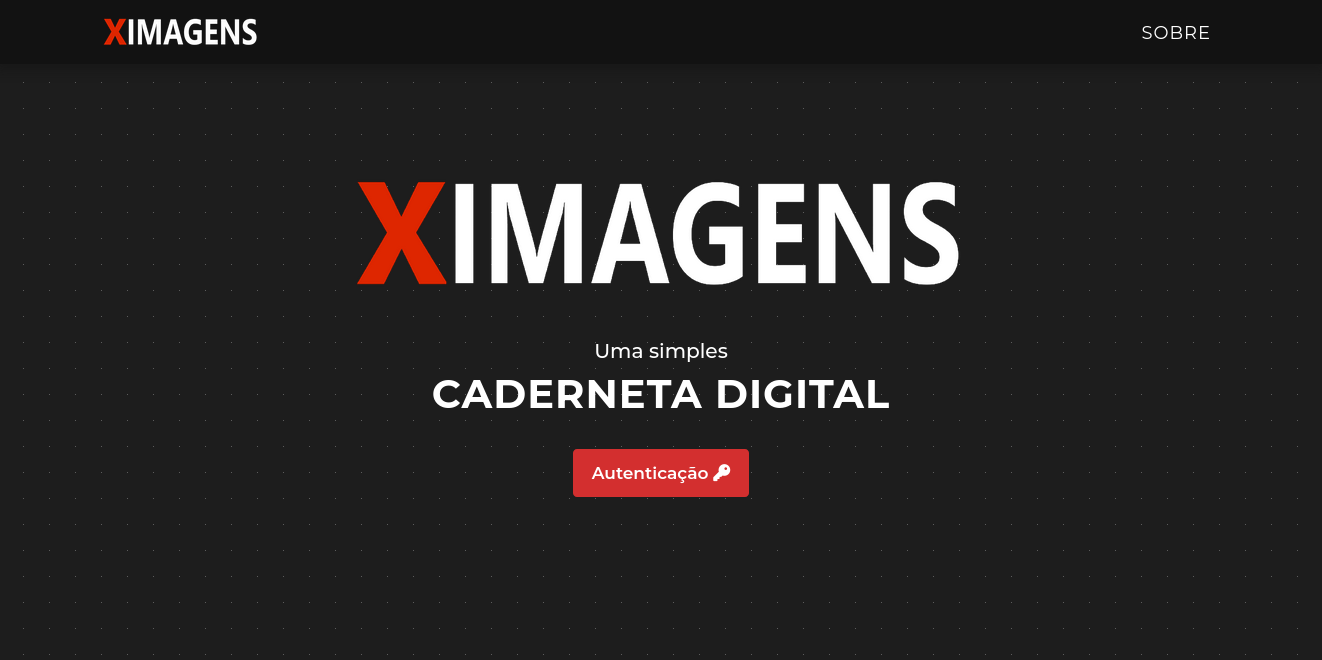
\includegraphics[width=\textwidth]{unknown.png}
    \caption{Página Inicial do site}
\end{figure}


\chapter{Persistência}
Este constituinte é composto por uma base de dados que permite o registo de informação. Estes métodos serão utilizados pela Aplicação Web ra registar uma referência para as imagens enviadas e os respetivos utilizadores que as possuem. 

A base de dados utilizada é a SQLite3, localizada no diretório da aplicação. O sistema armazena também  os ficheiros contendo as imagens, por outras palavras a base de dados terá informação sobre a data de inserção, comentários e outras propriedades, porém o ficheiro em si não é armazenado na base de dados.


\chapter{Processador de imagens}
Esta componente é executada como complementar à componente da aplicação web, e tem como principal função formatar e armazenar uma imagem que seja enviada pelo utilizador na aba de "Carregar" presente na NavBar.

O servidor irá reecber a imagem, reconhecer o seu conteúdo e tamanho e através duma implementação feita, irá aplicar uma marca de água na imagem com o intuito de a tornar autentica. Esta marca de água irá conter o logo do nosso site de modo a que a imagem continue a ser preceptivel para os utilizadores.
Esta marca de água além de informar que a imagem é verificada pelo nosso site, também irá indicar o dono da mesma, pois logo após a requisição duma imagem, será também aplicada na marca de água o nome de utilizador do dono da imagem.

Todas estas implementações ajudam na segurança do site, para não haver burlas nem roubos de imagens.

\begin{figure}[H]
    \centering
    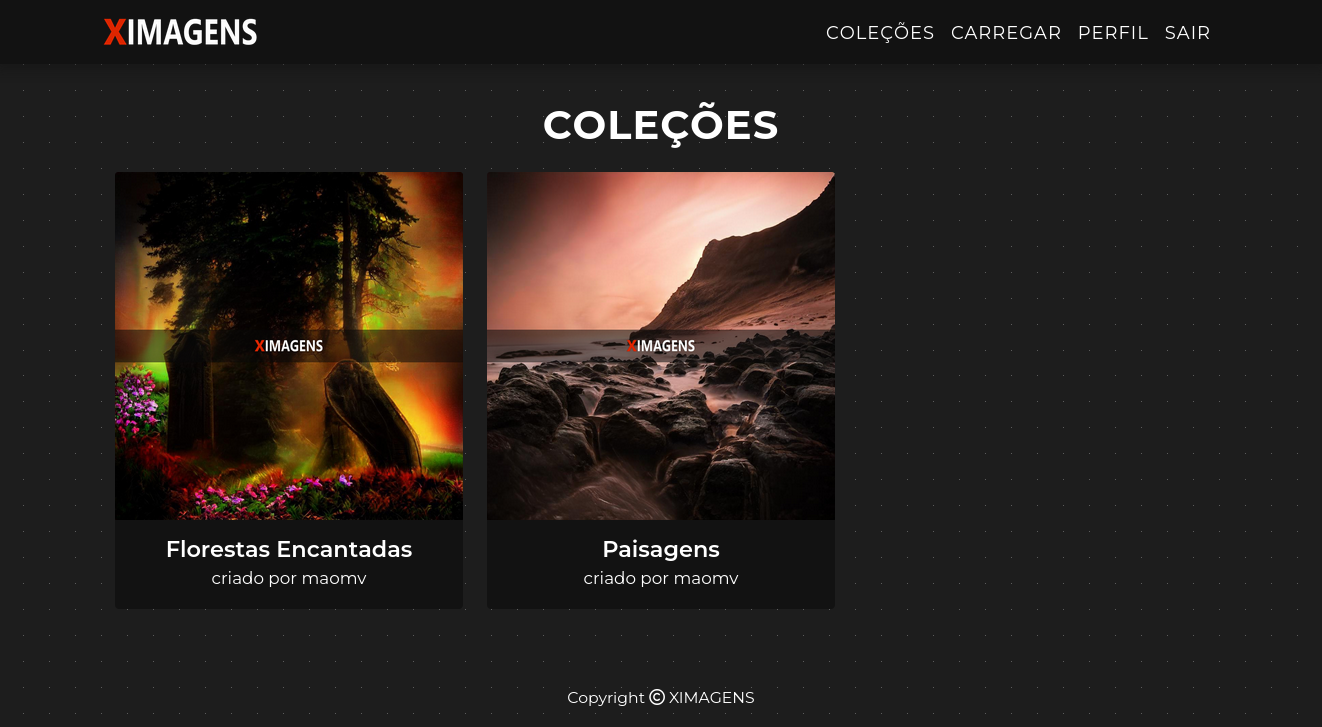
\includegraphics[width=\textwidth]{colecoes.png}
    \caption{Página das coleções do utilizador com a Marca de Água}
\end{figure}

\begin{figure}[H]
    \centering
    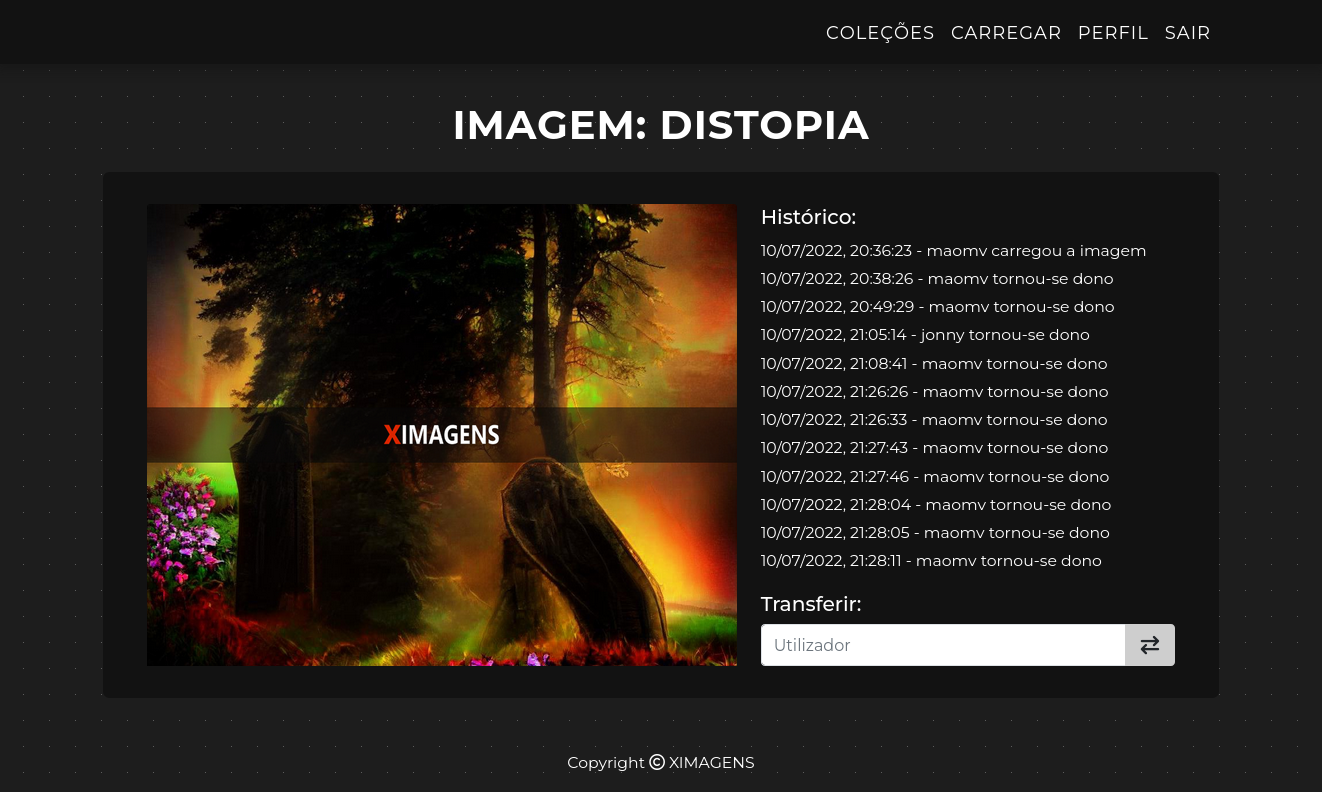
\includegraphics[width=\textwidth]{history.png}
    \caption{Página com o histórico a quem ja pertenceu a imagem}
\end{figure}



\chapter{Contribuições dos autores}
Durante este trabalho foi notório o esforço e dedicação de todos os participantes para a obtenção de um melhor resultado final. Várias horas de trabalho de grupo foram dispendidas para concluir o trabalho dentro dos prazos e com tudo funcional da melhor maneira possivel, ou seja, um site intuitivo, aparencia apelativa e totalmente funcional.

Por isso, consideramos que toda a gente ajudou de igual maneira à concretização do trabalho, ficando cada um com 25\% de participação no projeto.

Miguel Vila nMEC:107276; Diogo Silva nMEC:108212; Miguel Reis nMEC:108545; Martim Carvalho nMEC:108749;


\end{document}